% This is samplepaper.tex, a sample chapter demonstrating the
% LLNCS macro package for Springer Computer Science proceedings;
% Version 2.20 of 2017/10/04
%
\documentclass[runningheads]{llncs}
%

\usepackage{graphicx}
\graphicspath{ {\string~/Documents/retele_tema2/retele_pics} }

% Used for displaying a sample figure. If possible, figure files should
% be included in EPS format.
%
% If you use the hyperref package, please uncomment the following line
% to display URLs in blue roman font according to Springer's eBook style:
% \renewcommand\UrlFont{\color{blue}\rmfamily}

\begin{document}
%/Users/teodorciripescu
\title{Offline Messenger (B)}
%
%\titlerunning{Abbreviated paper title}•
% If the paper title is too long for the running head, you can set
% an abbreviated paper title here
%
\author{Ciripescu Teodor\\
\email{teodor.ciripescu@info.uaic.ro}\\}
%
% First names are abbreviated in the running head.
% If there are more than two authors, 'et al.' is used.
%
\institute{Facultatea de Informatica, UAIC\\
}
%
\maketitle              % typeset the header of the contribution
%
\begin{abstract}
Acest document contine planul de implementare pentru proiectul "Offline Messenger".

\end{abstract}
%
%
%
\section{Introducere}
%Sa se dezvolte o aplicatie client/server care sa permita schimbul de mesaje intre utilizatori care sunt conectati si sa ofere functionalitatea trimiterii mesajelor si catre utilizatorii offline, acestora din urma aparandu-le mesajele atunci cand se vor conecta la server. De asemenea, utilizatorii vor avea posibilitatea de a trimite un raspuns (reply) in mod specific la anumite mesaje primite. Aplicatia va oferi si istoricul conversatiilor pentru si cu fiecare utilizator in parte.
Aceasta abordare a proiectului Offline Messenger va avea in prim plan dezvoltarea unor sisteme de: autentificare/inregistrare a utilizatorilor, ”prietenie” intre utilizatori, stocare/procesare a conversatiilor dintre utilizatori, notificari din partea serverului in legatura cu anumite evenimente.\\
\section{Tehnologiile utilizate}
Vom utiliza un server TCP concurent cu threaduri. Pentru fiecare client serverul va crea un thread prin intermediul caruia se va ocupa de citirea comenzilor primite de la client si formularea raspunsurilor inapoi catre acesta. Pe cealalta parte, clientul va folosi 2 threaduri simultan. Unul pentru trimiterea de comenzi catre server si unul pentru citirea raspunsurilor de la acesta. Astfel, vom avea o comunicare fluenta client-server si server-client.\\
Am ales TCP datorita nevoiei unui protocol orientat spre conexiune si asigurarea transmiterii datelor intre cei ce comunica.\\
De asemenea, am ales folosirea threadurilor pentru ca sunt mai eficiente, mai lightweight decat o abordare cu procese copil. Mai mult, natura proiectului implica prezenta multor clienti conectati la server in acelasi timp, cat si citiri/scrieri  constante la server. Taskurile date serverului sunt in general simple si multe, deci se preteaza mai bine pe modelul cu threaduri.\\
Pentru stocarea utilizatorilor, relatiilor de prietenie si mesajelor va fi folosita o baza de date sqlite. 
Se va utiliza biblioteci precum sqlite3.h, pthread.h, socket.h, string.h .\\
\section{Arhitectura Aplicatiei}
\subsection{Ideea proiectului are la baza 5 componente}
-Autentificarea/Inregistrarea utilizatorilor\\
La inregistrare clientul isi alege un username (unic) si o parola. Acestea vor fi stocate in baza de date sub tabela users. \\
La autentificare se va cere ca input un username si o parola, daca username-ul exista si daca parola data ca input coincide cu cea prezenta in baza de date, clientul este autentificat. Acum are acces la o serie de comenzi specifice utilizatorilor. \\
In cazul unor impedimente precum: cineva incearca sa se inregistreze cu un username deja existent, parola scrisa la autentificare este gresita etc ..., clientul va fi atentionat de catre server.\\
-Sistem de "Prietenie" intre utilizatori\\
Fiecare utilizator autentificat va putea trimite cereri de prietenie catre alti utilizatori. In cazul in care aceste cereri sunt acceptate, vor putea incepe conversatii intre utilizatorii respectivi. \\
Utilizatorii vor putea sa isi vada lista de prieteni, sa trimita cereri de prietenie, sa isi vada lista cererilor de prietenie primite si sa accepte sau sa refuze cererile de prietenie.\\
-Procesarea/Stocarea Conversatiilor\\
Un client autentificat poate trimite altor clienti din lista sa de prieteni mesaje. Aceste mesaje vor avea asociate in baza de date campuri precum time, seen si reply\_to pentru a determina cand a fost trimis un mesaj, daca a fost vazut destinatar si daca reprezinta o replica la alt mesaj. Mesajele vor avea optiunea de a fi sterse.\\
-Notificari\\
Utilizatorii vor fi notificati de catre server cand au loc anumite evenimente: mesaj nou primit, cerere noua de prietenie, daca un mesaj a fost citit de catre destinatar. De asemenea, in momentul autentificarii, clientii vor fi atentionati de mesajele si cererile de prietenie pe care le-au primit pe perioada in care au fost offline.\\
\subsection{Protocolul}
Fiecare client va avea asociat threadul lui pe server si o structura in care va fi memorat descriptorul, username-ul si ID-ul de utilizator obtinut la autentificare. Threadul va inceta sa mai existe in momentul in care clientul se deconecteaza de la server. \\
Cand un client doreste sa se adreseze serverului acesta va trimite urmatoarele:\\
- 4 bytes pentru codul comenzii\\
- 2 bytes pentru lungimea mesajului\\
- mesajul propriu-zis cu lungimea anterior obtinuta\\
Cand serverul raspunde clientului trimite:\\
- 4 bytes pentru codul comenzii la care raspunde\\
- 2 bytes lungimea raspunsului\\
- raspunsul propriu-zis cu lungimea obtinuta anterior\\
Fiecare raspuns in parte poate fi format din mai multi parametri in functie de comanda.\\
Raspunsurile pot avea urmatoarele forme: \\
- 1 byte lungime parametru1, parametru1, 1 byte lungime parametru2, parametru2,...\\
- 1byte lung parametru1, 1 byte lung parametru2, …,parametru1, parametru2,...\\
In proiect sunt implementate momentan in jur de 20 de comenzi ce sunt numerotate in ordine de la 1 la 20. Cand un client apeleaza la server cu o comanda, acesta ii raspunde cu un acelasi cod de comanda. Sunt totusi unele cazuri in care serverul poate folosi un alt cod de comanda (erori, nevoia executiei unei comenzi precum seen,..).\\
Avem urmatoarele comenzi:\\
-login: are ca parametri username si password si are rol de autentificare a utilizatorului. In urma unei autentificari de succes, id-ul de utilizator si numele acestuia sunt salvate in memoria serverului. Acum clientul capata acces la alte comenzi ce sunt specifice utilizatorilor autentificati.\\
-register: are ca parametri username si password, inregistreaza clientul in baza de date. Aceasta returneaza daca inregistrarea a avut loc cu succes.\\
-getFriendList: nu are niciun parametru si returneaza numele utilizatorilor cu care suntem “prieteni”\\
-sendFriendRequest: are ca parametrul username-ul utilizatorului cu care vrem sa fim prieteni. Se va consemna in baza de date aceasta intentie.\\
-acceptFriendRequest(param: username): prin aceasta comanda se accepta cererile de prietenie primite. Odata acceptata, se poate incepe conversatia intre utilizatori.\\
-rejectFriendRequest(param: username): se respinge cererea de prietenie.\\
-getMessages(params:username, nr\_mesaje): vor fi extrase din baza de date si trimise clientului un anumit numar de mesaje din conversatia cu un utilizator. Mesajele, pe langa continutul efectiv, contin si detalii precum momentul la care au fost trimise, daca au fost vazute sau nu si daca reprezinta o replica la un alt mesaj.\\
-getUnseenMessages(params:username): ne vor fi afisate mesajele pe care inca nu le-am vazut de la un anumit utilizator. De mentionat ca la autentificare, fiecare utilizator este notificat de la cine si cate mesaje nevazute are.\\
-sendMessage(params:username, mesaj): clientul trimite mesajul la server, acesta este incarcat in baza de date, si trimis destinatarului in cazul in care acesta este online. De asemenea, vom fi notificati daca acesta este sau nu online si daca a vazut mesajul.\\
-replyMessage(username, mesaj, id\_mesaj\_replica) acesta comanda ne da posibilitatea de a marca un mesaj ca fiind un raspuns (reply) la un alt mesaj din conversatie.\\
-deleteMessage(id\_mesaj): ne da posibilitatea de a sterge un anumit mesaj\\
-logout(fara parametri): aceasta functie elimina conexiunea dintre server si client.\\
-seen(param:id\_mesaj): comanda este apelata automat de catre client in momenul in care acesta a vazut un mesaj. Cel care a trimis mesajul, este atentionat de acest lucru.\\
-getFriendListPendingMessages(fara parametri): ni se afiseaza o lista cu cei ce ne-au trimis mesaje dar si numarul lor.\\
\bigskip\\
Diagrama generala:\\
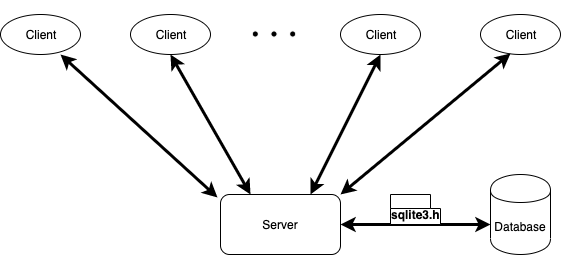
\includegraphics[width=100mm,scale=1]{retele_pics/general_diagram.png}\\
Diagrama clase server:\\
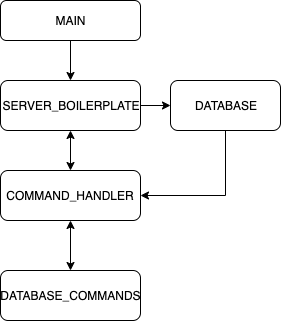
\includegraphics[width=50mm,scale=1]{retele_pics/server_classes.png}\\
Diagrama clase client:\\
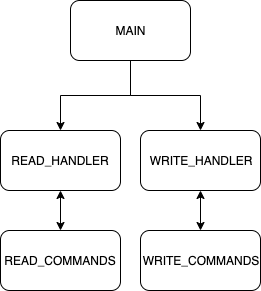
\includegraphics[width=50mm,scale=1]{retele_pics/client_classes.png}\\
Vom folosi o baza de date sqlite pe care o vom accesa prin intermediul bibliotecii sqlite3.h . Toate apelurile catre baza de date vor fi facute de catre server in urma comenzilor date de catre clienti.\\
Baza de date va respecta urmatoarea schema:\\
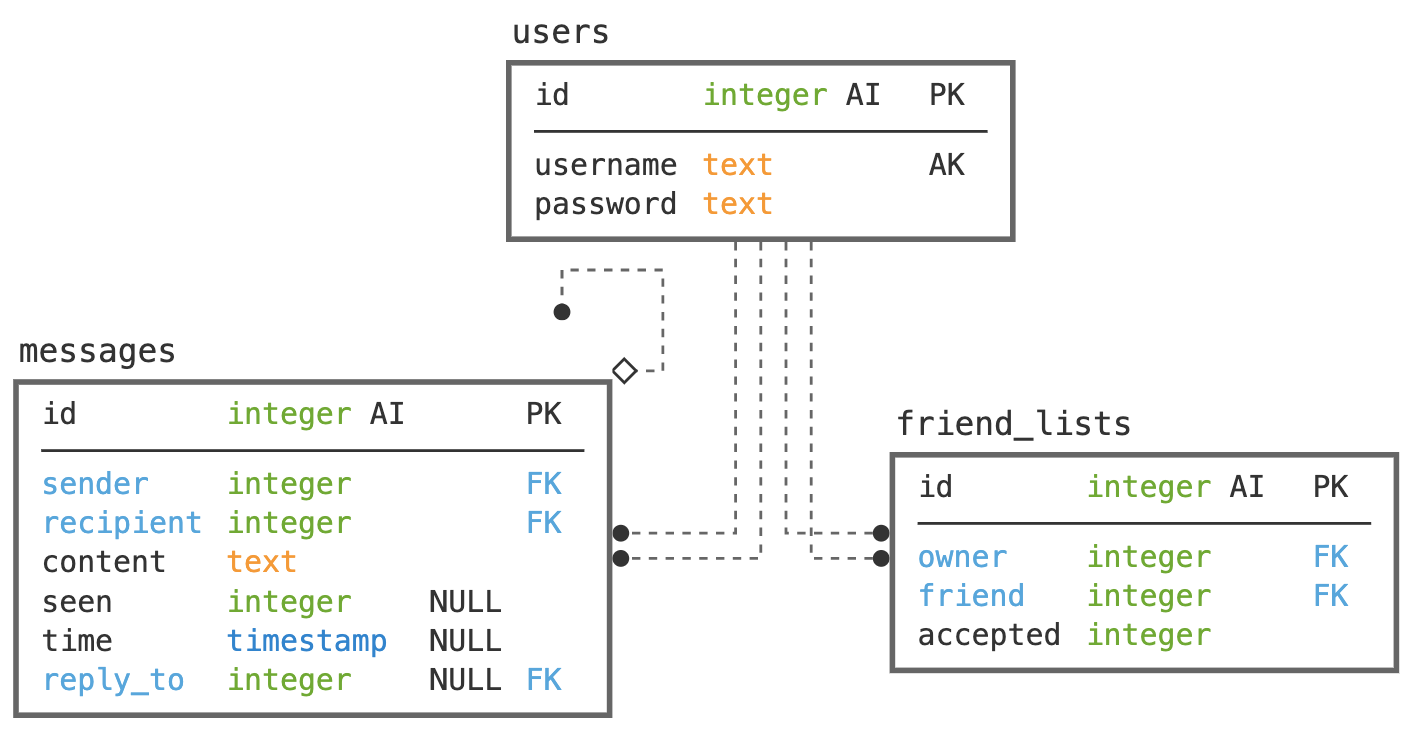
\includegraphics[width=150mm,scale=1]{retele_pics/database_schemas/database_schema.png}\\
\section{Detalii de implementare}
-Serverul va face toate schimbarile in baza de date in urma comenzilor date de catre utilizatori. Acesta va fi singurul care se va conecta direct la baza de date. Clasa database\_commands contine toata functiile ce fac query pe baza de date.\\
-In lista de prieteni va fi inregistrata prietenia din ambele sensuri. Fiecare in parte trebuie sa aiba acceptata “prietenia” (poti sterge pe cineva ca prieten si el sa te aiba in continuare in lista dar sa nu iti poata trimite mesaje).\\
-Cand un client incerca sa trimita un mesaj catre alt client, se va face o verificare daca cei doi sunt prieteni. In caz afirmativ, mesajul este trimis.
-Serverul are un sistem de management al utilizatorilor conectati cu functii de adaugare, stergere si gasire a structurilor asociate userilor:\\
addThreadData(...), deleteThreadData(...), printThreadData(), getDescriptorFromOnlineUser(...), getDescriptorFromOnlineUser(...)\\
-Daca clientul se deconecteaza atat intr-un mod normal cat si printr-o maniera neasteptata, serverul va sterge datele clientului referitoare la acea sesiune (descriptorul, id-ul userului)\\
-Cand un utilizator cere sa vada mesajele dintr-o anumita conversatie, serverul trimite mesajele in mai multe pachete in functie de numarul lor.(un pachet contine 10 mesaje)\\


\section{Concluzii si posibile aditii}
Luand in considerare cele de mai sus putem intelege ca orice request al unui client catre server are urmatorulu drum. In prima instanta, clientul se conecteaza la server si un thread ii este alocat pentru managementul requesturilor. Detalii referitoare la client vor fi retinute intr-o structura de tipul thData (descriptorul si id-ul care initial este -1 din lipsa de autentificare). Acum singurele comenzi ce pot fi facute de catre client sunt register si authenticate. In urma unei autentificari cu succes (ce implica o interogare a bazei de date cu parametrii username si password), campului idUser din structura thData ii este atribuita valoarea id-ului asociat utilizatorului din tabela users a bazei de date. Clientul capata mai multe drepturi, si anume accesul la mai multe comenzi(prezentate mai sus). Proaspat autentificat, utilizatorul este notificat de ce a ratat in perioada in care a fost offline (mesaje noi, cereri de prieteni). Noi cereri de prietenie si mesaje noi vor aparea in continuare pe parcursul rularii.\\
In momentul in care un client doreste sa trimita un mesaj altui client, acesta va folosi una dintre functiile de trimitere mesaj catre server. Serverul va cauta in vectorul de structuri thData descriptorul destinatarului si ii va transmite mesajul prin acesta.\\
Un feature necesar pentru securitate este stocarea parolelor sub forma de hashuri in baza de date. La autentificare se va face o comparare de hashuri.
Poate fi implementata si o solutie de criptare a mesajelor. Va trebui folosita o metoda de a securiza schimbul de chei ( Diffie Hellman key exchange).\\
\begin{thebibliography}{8}
\bibitem{ref_article1}
https://www.sqlite.org/whentouse.html
\bibitem{ref_article1}
https://www.sqlite.org/capi3ref.html
\bibitem{ref_article1}
https://profs.info.uaic.ro/~computernetworks/files/NetEx/S12/ServerConcThread/servTcpConcTh2.c
\bibitem{ref_article1}
https://profs.info.uaic.ro/~computernetworks/files/NetEx/S12/ServerConcThread/cliTcpNr.c
\bibitem{ref_article1}
https://www.geeksforgeeks.org/sql-using-c-c-and-sqlite/
\end{thebibliography}
\end{document}
